

\documentclass{article}
\usepackage{CJK}
\usepackage{amsmath,amssymb}
\usepackage{fancyhdr}  
\usepackage{graphicx}
\usepackage{float}


\begin{document}
\begin{CJK*}{GBK}{song}

\pagestyle{fancy}  
\fancyhead{} % clear all fields  
\fancyhead[R]{Data Analysis}  
\fancyhead[L]{Chenxi Gu\\ 2017311017} 
\renewcommand{\headrulewidth}{0.4pt}  
\renewcommand{\footrulewidth}{0.4pt} 



\title {chapter 4}
\author{Chenxi Gu\\2017311017}

\date{\today}

\maketitle
\section{4.1}
(a)
Significance level $\alpha=0.1737$\\
(b)
Power $1-\beta=0.8263$\\
\begin{equation}
P_{\pi\rightarrow e}=0.1737
\end{equation}
(c)
\begin{equation}
P=\frac{0.01*0.8263}{0.01*0.8263+0.99*0.1737}=0.046
\end{equation}
(d)
\begin{equation}
\frac{0.01*\Phi(t)}{0.01*\Phi(t)+0.99*\Phi(t-2)}=0.95
\end{equation}
\begin{equation}
\begin{aligned}
&t=-2.5155\\
&\epsilon_e=0.005943\\
&\alpha=1-\epsilon_e=0.994057
\end{aligned}
\end{equation}

\section{4.2}
(a)
When $J(\textbf{a})$ have max value, satisfy $\frac{\partial J}{\partial a_i}=0$. We can get n equations such as:
\begin{equation}
\frac{\sum_j a_jw_{ij}}{(\mu_0-\mu_1)_i}=\frac{\sum_j a_j(\mu_0-\mu_1)_j\sum_{i,j} a_ia_jw_{ij}}{\sum_{i,j} a_ia_j(\mu_0-\mu_1)_i(\mu_0-\mu_1)_j}
\end{equation}
We find the right of the equation is a constant.So we make it equal $k$.
\begin{equation}
\textbf{a}=k\textbf{W}^{-1}(\boldsymbol{\mu}_0-\boldsymbol{\mu}_1)
\end{equation}
(b)
\begin{equation}
P(H_0|\textbf{x})=\frac{f(\textbf{x}|H_0)\pi_0}{f(\textbf{x}|H_0)\pi_0+f(\textbf{x}|H_1)\pi_1}=\frac{1}{1+\frac{\pi_1}{\pi_0r}}
\end{equation}
while $r=exp[(\boldsymbol{\mu}_0-\boldsymbol{\mu}_1)^TV^{-1}\textbf{x}-\frac{1}{2}\boldsymbol{\mu}_0^TV^{-1}\boldsymbol{\mu}_0+\frac{1}{2}\boldsymbol{\mu}_1^TV^{-1}\boldsymbol{\mu}_1]$\\
(c)
using (b) result :
\begin{equation}
\begin{aligned}
&t=In(\frac{\pi_0}{\pi_1})+In(r)\\
&a_0=In(\frac{\pi_0}{\pi_1})-\frac{1}{2}\boldsymbol{\mu}_0^TV^{-1}\boldsymbol{\mu}_0+\frac{1}{2}\boldsymbol{\mu}_1^TV^{-1}\boldsymbol{\mu}_1
\end{aligned}
\end{equation}

\section{4.3}
\begin{equation}
P=1-Poisson_{cdf}(15,3.9)=0.0000035797
\end{equation}


\section{4.4}
(a)
For two different theory:
\begin{equation}
\begin{aligned}
&\chi^2_1=15.8193\\
&\chi^2_2=35.9653
\end{aligned}
\end{equation}
\begin{figure}[H]
\centerline{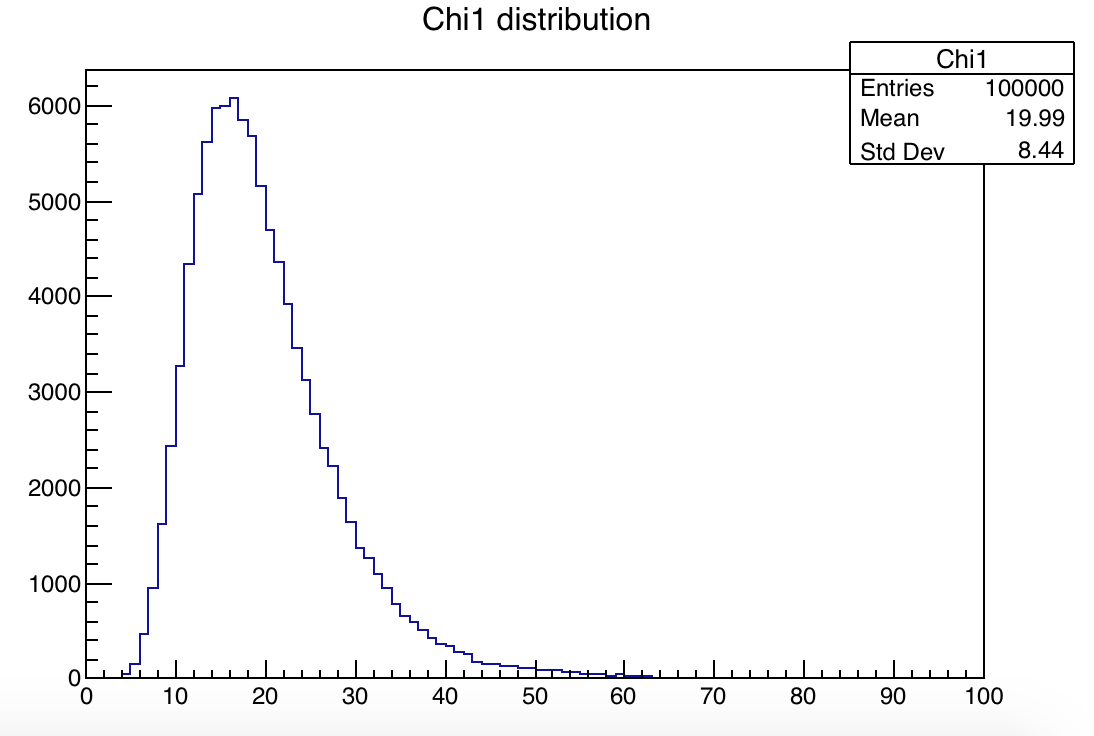
\includegraphics[scale=0.4]{4.4b1.png}}
\caption{Chi1 distribution}
\label{fig:label}
\end{figure}
\begin{figure}[H]
\centerline{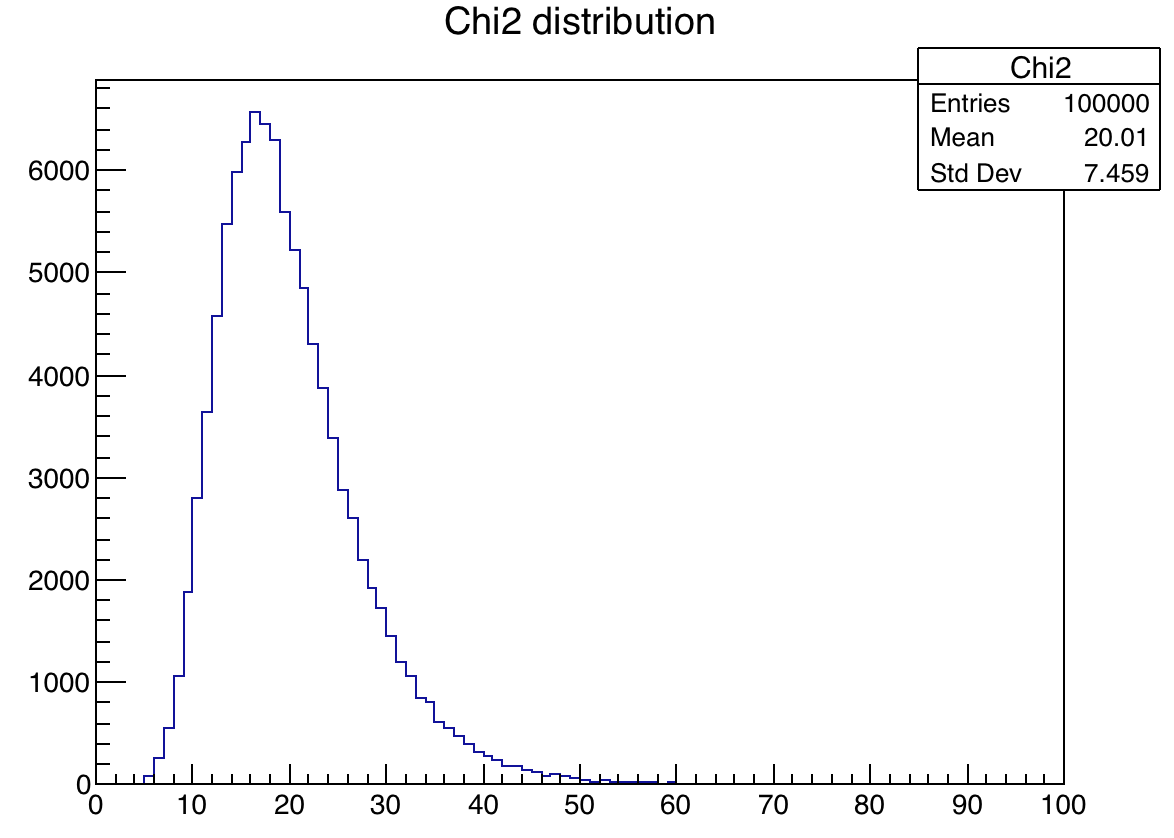
\includegraphics[scale=0.4]{4.4b2.png}}
\caption{Chi2 distribution}
\label{fig:label}
\end{figure}
We can calculate $P$ value using Chi1 and Chi2 distribution:
\begin{equation}
\begin{aligned}
&P_1=0.65251\\
&P_2=0.0353
\end{aligned}
\end{equation}

using $\chi^2$ distribution:
\begin{equation}
\begin{aligned}
&P_1^*=0.727769\\
&P_2^*=0.015526
\end{aligned}
\end{equation}


\section{4.5}
(a)
\begin{figure}[H]
\centerline{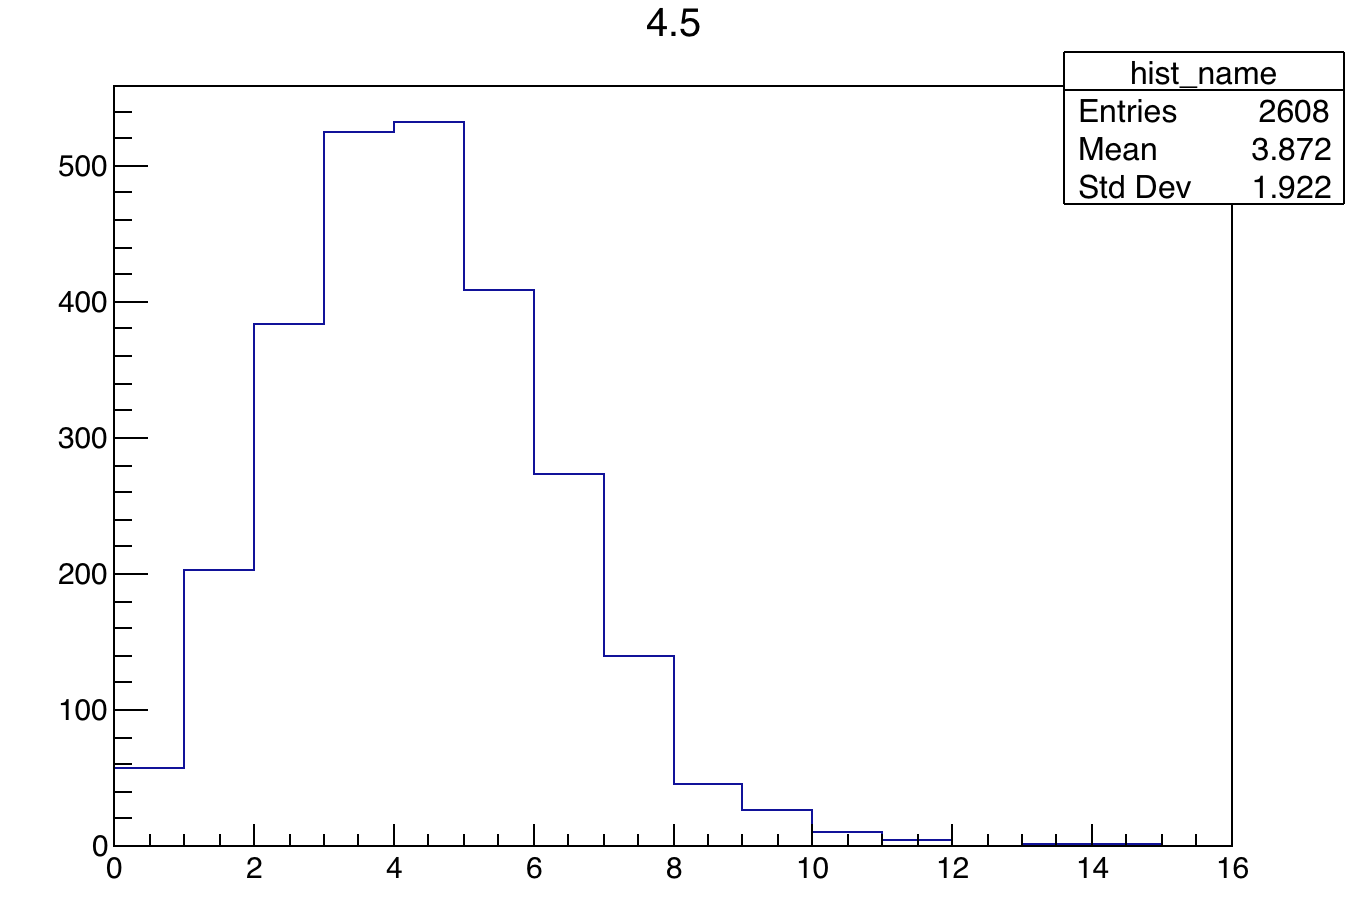
\includegraphics[scale=0.4]{4.5a.png}}
\caption{Data}
\label{fig:label}
\end{figure}
\begin{equation}
t=\frac{s^2}{\bar{m}}=0.954
\end{equation}
(b)If we use gaussian distribution:
\begin{equation}
P=0.951749
\end{equation}
We should let $t=1$ represent whether observations consistent with Poisson hypothesis.\\
(c)
\begin{figure}[H]
\centerline{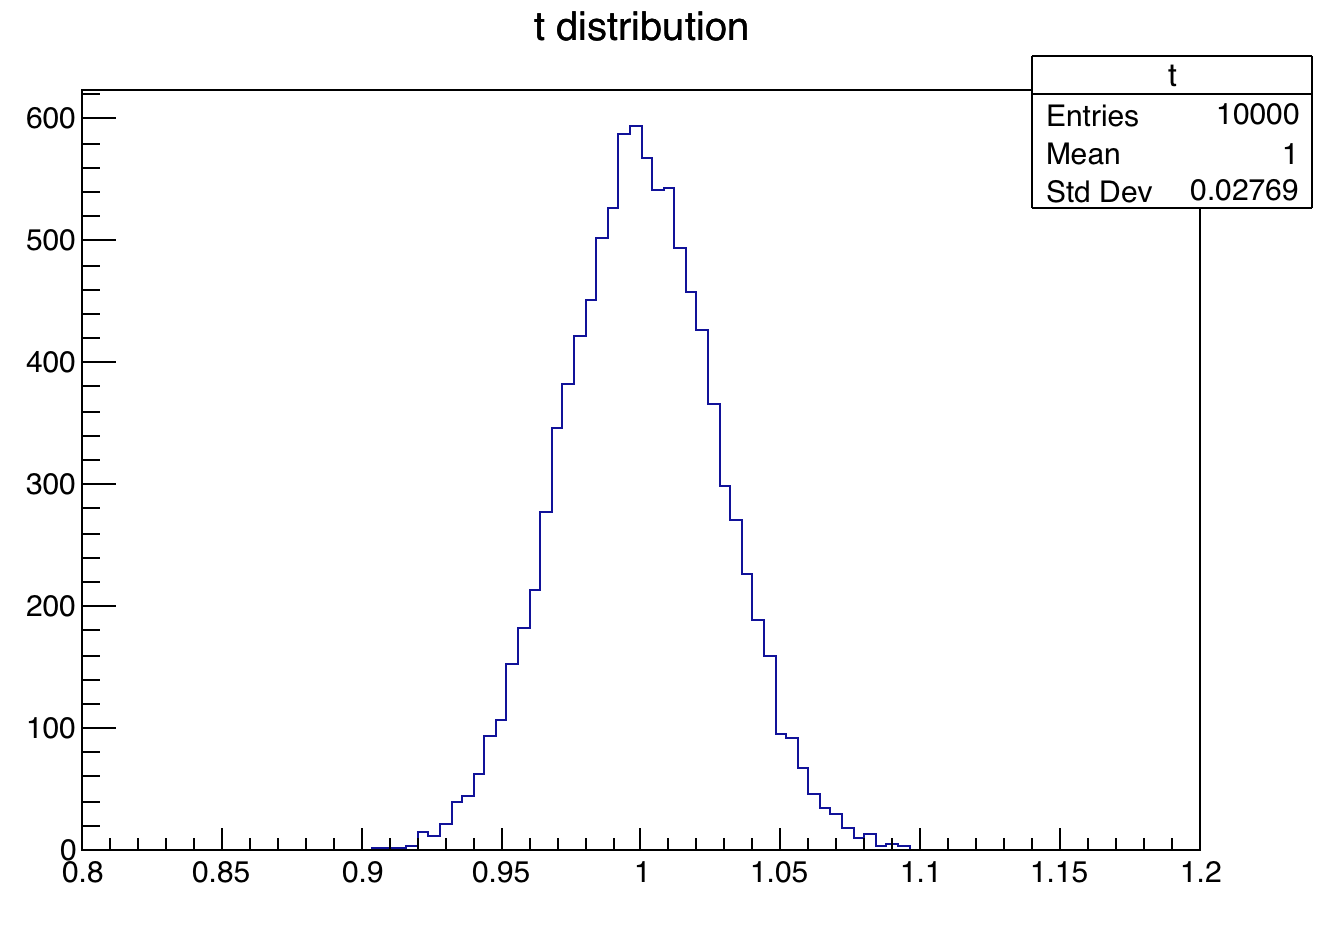
\includegraphics[scale=0.4]{4.5c.png}}
\caption{t distribution}
\label{fig:label}
\end{figure}

\begin{equation}
P=0.95268
\end{equation}






\end{CJK*}
\end{document}
